\documentclass[pdf,mathserifaspectratio=169]{beamer}
\usepackage[orientation=landscape,size=custom,width=16,height=9,scale=0.5,debug]{beamerposter}
\usepackage{etex}
\usetheme{ltg}

\usepackage{textcomp}
\usepackage{ifpdf}
\usepackage{pxfonts}
\usepackage[american]{babel} 
\usepackage[utf8]{inputenc}
\usepackage{lmodern}
\usepackage[T1]{fontenc}
\usepackage{relsize}
\usepackage{amsmath}
\usepackage{multirow}
\usepackage{booktabs}
\usepackage{colortbl}
\usepackage{xcolor}
\usepackage{thumbpdf}
\usepackage{graphicx}
\usepackage{fancybox}
\usepackage{hyperref}
\usepackage{textcomp}
\usepackage{pdfpages}
\usepackage{ulem}
\usepackage{tikz}
\usetikzlibrary{arrows,shapes,backgrounds}
\usepackage{pgfplots,pgfplotstable}
\usepackage{natbib}
\usepackage{apalike}
\bibliographystyle{apalike}

\newcommand{\ntuple}[2]{\ensuremath{\left({#1}_1, {#1}_2, \ldots, {#1}_{#2}\right)}}
\newcommand{\vect}[1]{\ensuremath{\boldsymbol{#1}}}
\newcommand{\mat}[1]{\ensuremath{\boldsymbol{#1}}}
\newcommand{\func}[1]{\ensuremath{\operatorname{{#1}}}}

\newcommand{\cf}{cf.}
\newcommand{\eg}{e.g.}
\newcommand{\ie}{i.e.}
\newcommand{\etc}{etc.}
\newcommand{\vs}{vs.}
\newcommand{\viz}{viz.}
\newcommand{\etal}{et al.}

\def\argmax{\mathop{\rm arg\,max}}
\def\argmin{\mathop{\rm arg\,min}}
\def\fscore{F$_1$}


\usepackage{latexsym}
\usepackage{graphics}
\usepackage{color}
\usepackage{fancyvrb}
\usepackage{adjustbox}

\usepackage{pifont}\newcommand{\cmark}{\ding{51}}\newcommand{\xmark}{\ding{55}}

\definecolor{oe}{rgb}{0,0,1}
\definecolor{DarkBlue}{rgb}{0.1,0.1,0.5}
\definecolor{LightGreen}{rgb}{0.1,0.5,0.1}
\definecolor{DarkGreen}{rgb}{0,0.2,0}
\definecolor{Red}{rgb}{0.9,0.0,0.1}
\definecolor{Dandelion}{cmyk}{0,0.25,0.84,0}
\definecolor{lgray}{gray}{0.85}
\definecolor{mgray}{gray}{0.4}
\definecolor{light}{gray}{.2}

\fboxsep 0pt
\pgfdeclareimage[height=8mm]{logo}{graphics/logo}
\pgfdeclareimage[height=8mm]{openeurollm}{graphics/openeurollm}
\usepackage[many]{tcolorbox}
\usepackage[absolute,overlay]{textpos}
\setlength{\TPHorizModule}{1mm}
\setlength{\TPVertModule}{1mm}
\newcommand{\includelogo}{%
  \textblockcolor{white}%
  \begin{textblock}{10}(153,0.25)\pgfuseimage{logo}\end{textblock}}
\newcommand{\includeopeneurollm}{%
  \begin{textblock}{10}(143.7,0.25)\pgfuseimage{openeurollm}\end{textblock}}

\begin{document}

\title[]{R\&D for (Open) Large Language Models in Norway}
\author[]{Stephan Oepen, Language Technology Group (LTG, University of Oslo\\ \vskip -4ex}
\date[]{\color{DarkBlue}September 29, 2026 -- NorwAI Innovate at the Trondheim Tech Festival}
\institute[]{}

%\iffalse
\begin{frame}[fragile,plain]
  \vskip -1ex
  \centerline{
\includegraphics[height=28mm]{graphics/logo+name}}
  \vskip -2ex
  \titlepage
\end{frame}

\begin{frame}[fragile,plain]
  \begin{columns}
    \begin{column}{0.4\textwidth}
      \vspace*{-8ex}
      \begin{center}
        \fontsize{7cm}{7cm}\selectfont\bfseries 0
      \end{center}      
    \end{column}
    \begin{column}{0.65\textwidth}
      \begin{center}\renewcommand{\baselinestretch}{1.5}
        \fontsize{1.1cm}{1.1cm}\selectfont\bfseries
        Background,\\ Preliminaries
      \end{center}
    \end{column}
  \end{columns}
\end{frame}

\begin{frame}[fragile]\includelogo
  \frametitle{Language Models, Cultural Identity, Digital Sovereignty}
  \vskip 0ex
  \begin{columns}
    \begin{column}{.76\textwidth}
      \begin{center}
        
\includegraphics[width=.22\textwidth]{graphics/chatgpt}\hskip 2em
        
\includegraphics[width=.22\textwidth]{graphics/copilot}\hskip 2em
        
\includegraphics[width=.22\textwidth]{graphics/claude}
      \end{center}
      \pause
      \begin{block}{Språklig og kulturell identitet}
        \begin{itemize}\itemsep 4pt\itshape
          \item I helg\alert<3>{en} var \alert<2>{jeg} på hytt\alert<3>{en} i \alert<2>{skogen} og dans\alert<3>{et} med \alert<4>{min \alert<2>{søster}}.
          \item I helg\alert<3>{a} var \alert<2>{jeg} på hytt\alert<3>{a} i \alert<2>{skauen} og dans\alert<3>{a} med \alert<4>{\alert<2>{søster}a mi}. 
          \item I helg\alert<3>{a} var \alert<2>{eg} på hytt\alert<3>{a} i \alert<2>{skogen} og dans\alert<3>{a} med \alert<4>{\alert<2>{syster}a mi}. 
          \item I helg\alert<3>{a} var \alert<2>{eg} på hytt\alert<3>{a} i \alert<2>{skogen} og dans\alert<3>{a} med \alert<4>{\alert<2>{søster}a mi}. 
        \end{itemize}
      \end{block}
    \end{column}
    \pause\pause\pause
    \begin{column}{.24\textwidth}
      \begin{center}\fboxsep 0pt
        \fbox{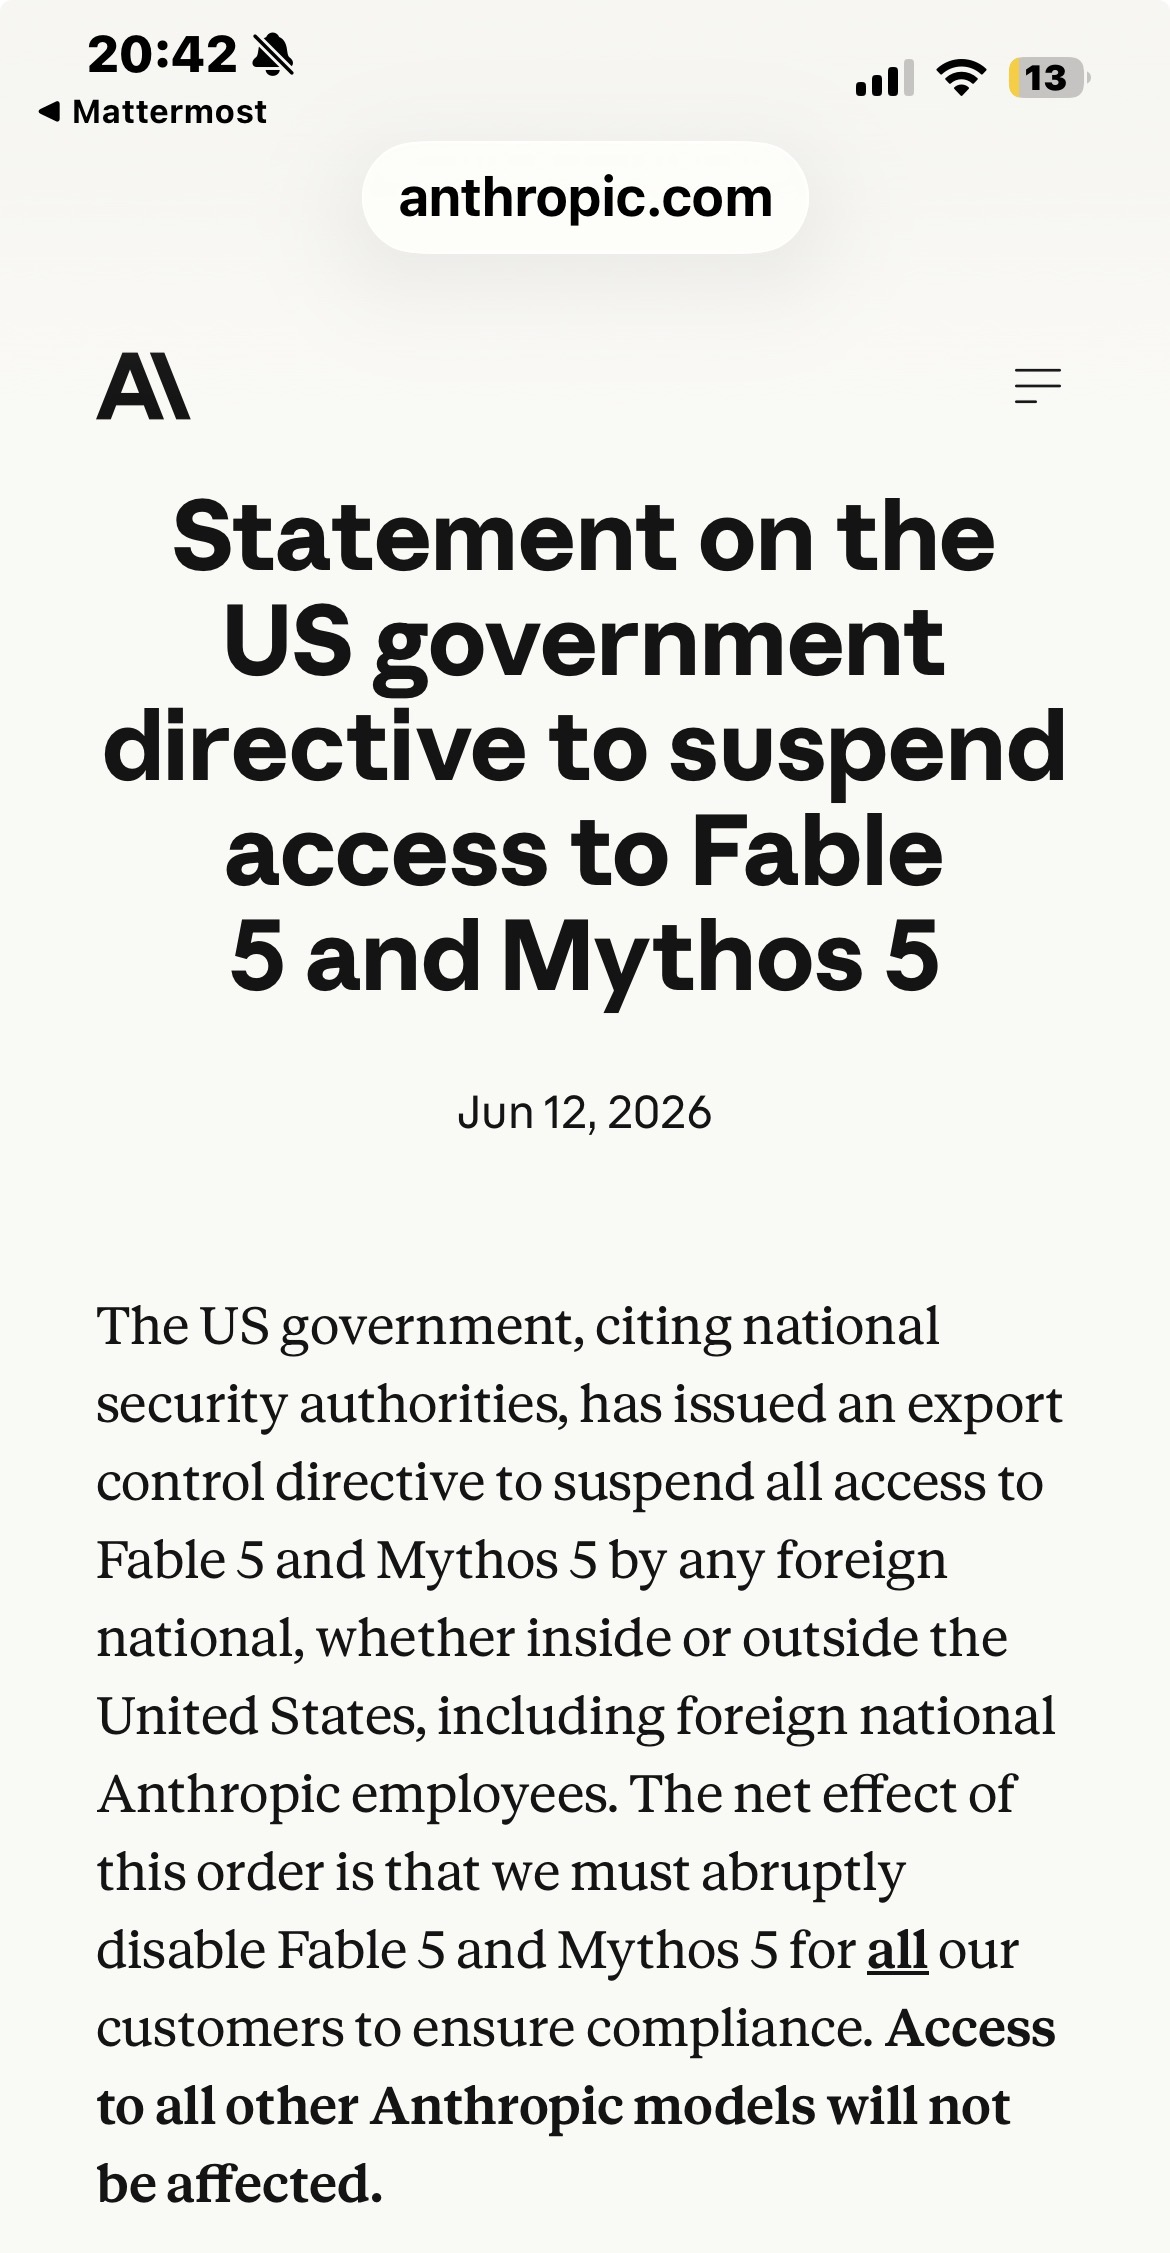
\includegraphics[width=.94\textwidth]{graphics/anthropic}}\\[1.5ex]
      \end{center}
    \end{column}
  \end{columns}
\end{frame}

\begin{frame}[fragile]\includelogo
  \frametitle{By Way of Self-Introduction (Gemma-4-21b-it)}
  \pause
  \vskip -3ex
  \begin{center}
    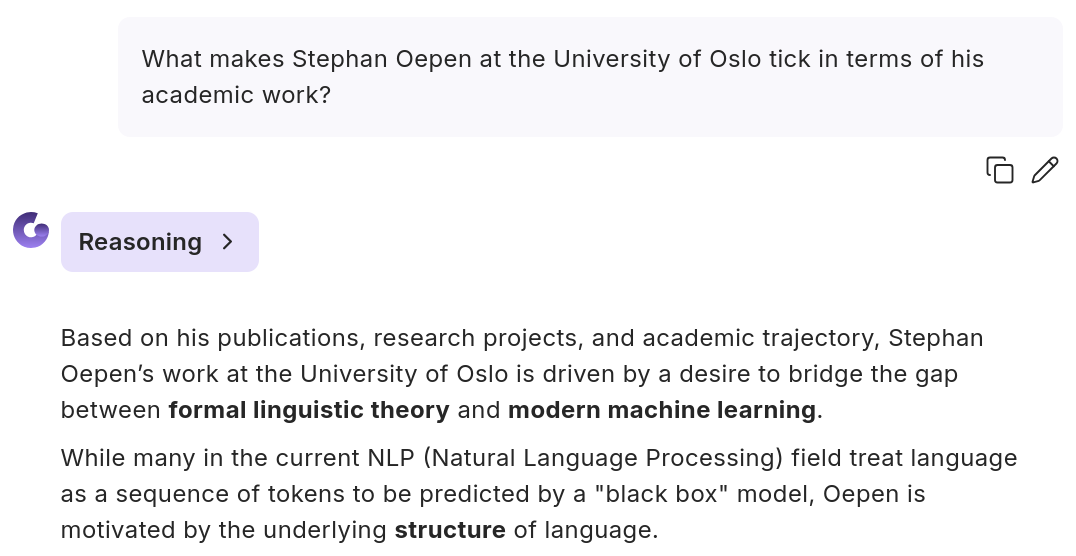
\includegraphics[width=0.75\textwidth, trim={0cm 0cm 0cm .8cm}, clip]{graphics/gemma4-oepen-1}\\[-1ex]
    \pause
    {\larger\textbf{\ldots}}\\[1.25ex]
    \hskip 2.5ex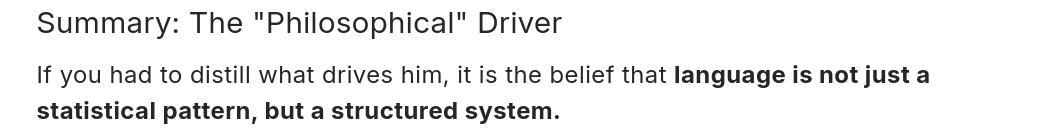
\includegraphics[width=0.75\textwidth]{graphics/gemma4-oepen-2}
  \end{center}
\end{frame}

\begin{frame}[fragile]\includelogo
  \frametitle{``Hallucination'' Remains a Challenge}
  \begin{columns}
    \begin{column}{0.72\textwidth}
      \vskip -3ex
      \begin{center}
        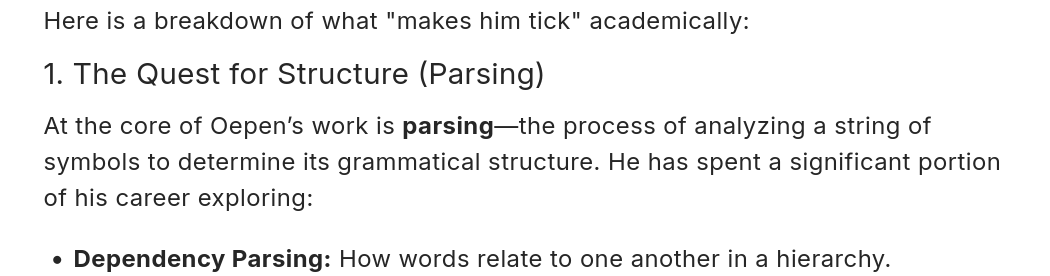
\includegraphics[width=\textwidth]{graphics/gemma4-oepen-3}\\[-1ex]
        \pause
        {\larger\textbf{\ldots}}\\[.75ex]
        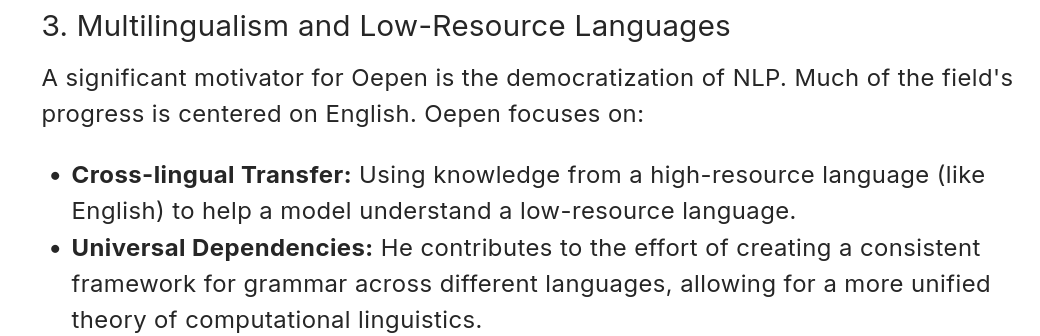
\includegraphics[width=\textwidth]{graphics/gemma4-oepen-4}
      \end{center}
    \end{column}
    \pause
    \begin{column}{0.28\textwidth}
      \begin{center}
        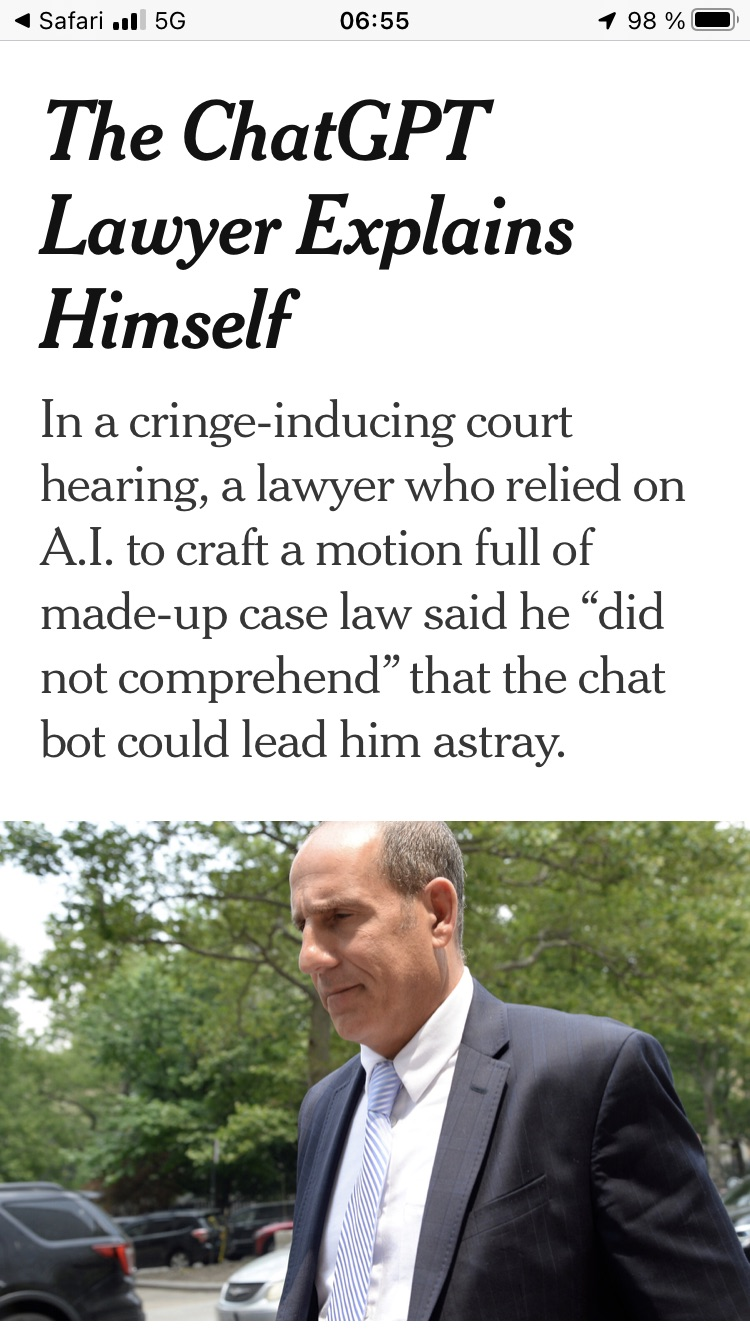
\includegraphics[width=\textwidth]{graphics/schwartz.jpg}
      \end{center}
    \end{column}
  \end{columns}
\end{frame}

\begin{frame}[fragile,plain]
  \begin{columns}
    \begin{column}{0.4\textwidth}
      \vspace*{-8ex}
      \begin{center}
        \fontsize{7cm}{7cm}\selectfont\bfseries 1
      \end{center}      
    \end{column}
    \begin{column}{0.65\textwidth}
      \begin{center}\renewcommand{\baselinestretch}{1.5}
        \fontsize{1.1cm}{1.1cm}\selectfont\bfseries
        The Situation\\ in Norway
      \end{center}
    \end{column}
  \end{columns}
\end{frame}

\begin{frame}[fragile]\includelogo
  \frametitle{Februar 5:\ Renewed and Intensified Collaboration}
  \vskip -1ex
  \begin{columns}
    \begin{column}{.7\textwidth}
      \begin{center}
        \fbox{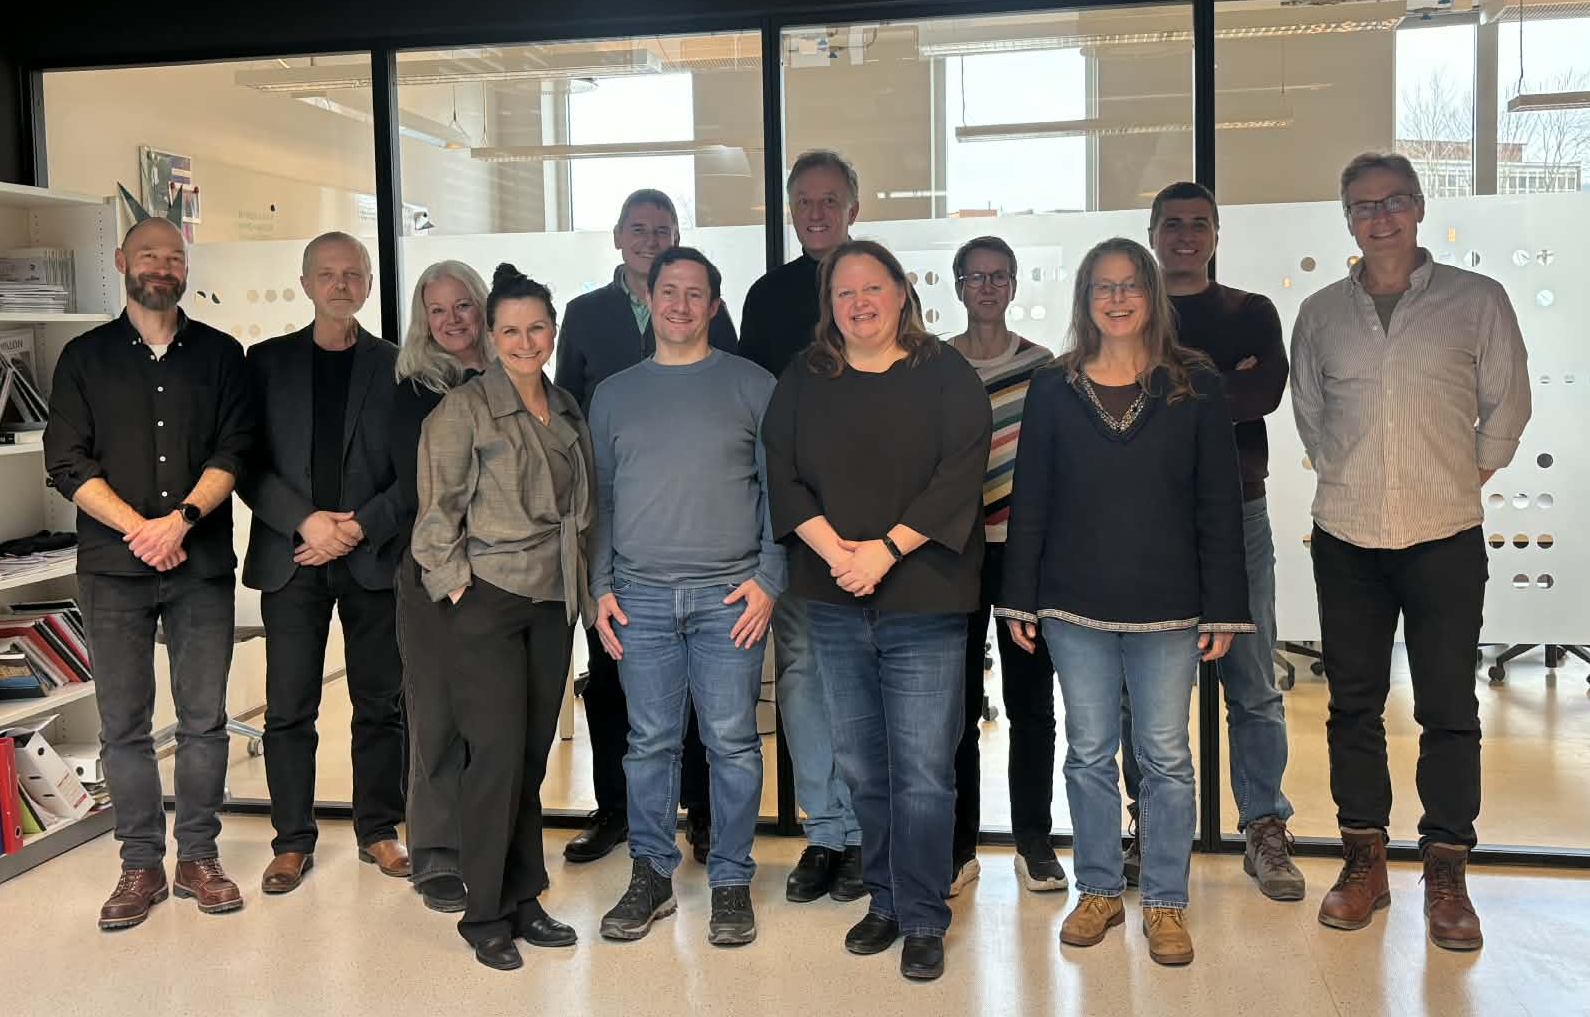
\includegraphics[width=.95\textwidth]{graphics/260205}}\\[1.5ex]
      \end{center}
    \end{column}
%    \pause
    \begin{column}{.3\textwidth}
      \begin{center}
        
\includegraphics[width=.95\textwidth]{graphics/nb.png}\\[1.5ex]
        
\includegraphics[width=.94\textwidth]{graphics/ntnu}\\[1.5ex]
        
\includegraphics[width=.95\textwidth]{graphics/uio}\\[2.5ex]
%        \pause
        
\includegraphics[width=.93\textwidth]{graphics/sigma2}\\[1.5ex]
        
\includegraphics[width=.95\textwidth]{graphics/lcn}\\
      \end{center}
    \end{column}
  \end{columns}
\end{frame}

\iffalse
\begin{frame}[fragile]\includelogo
  \frametitle{2024:\ M\'imir-oppdraget fra Kulturdepartementet}
  \vskip -4ex
  \begin{center}
    \fbox{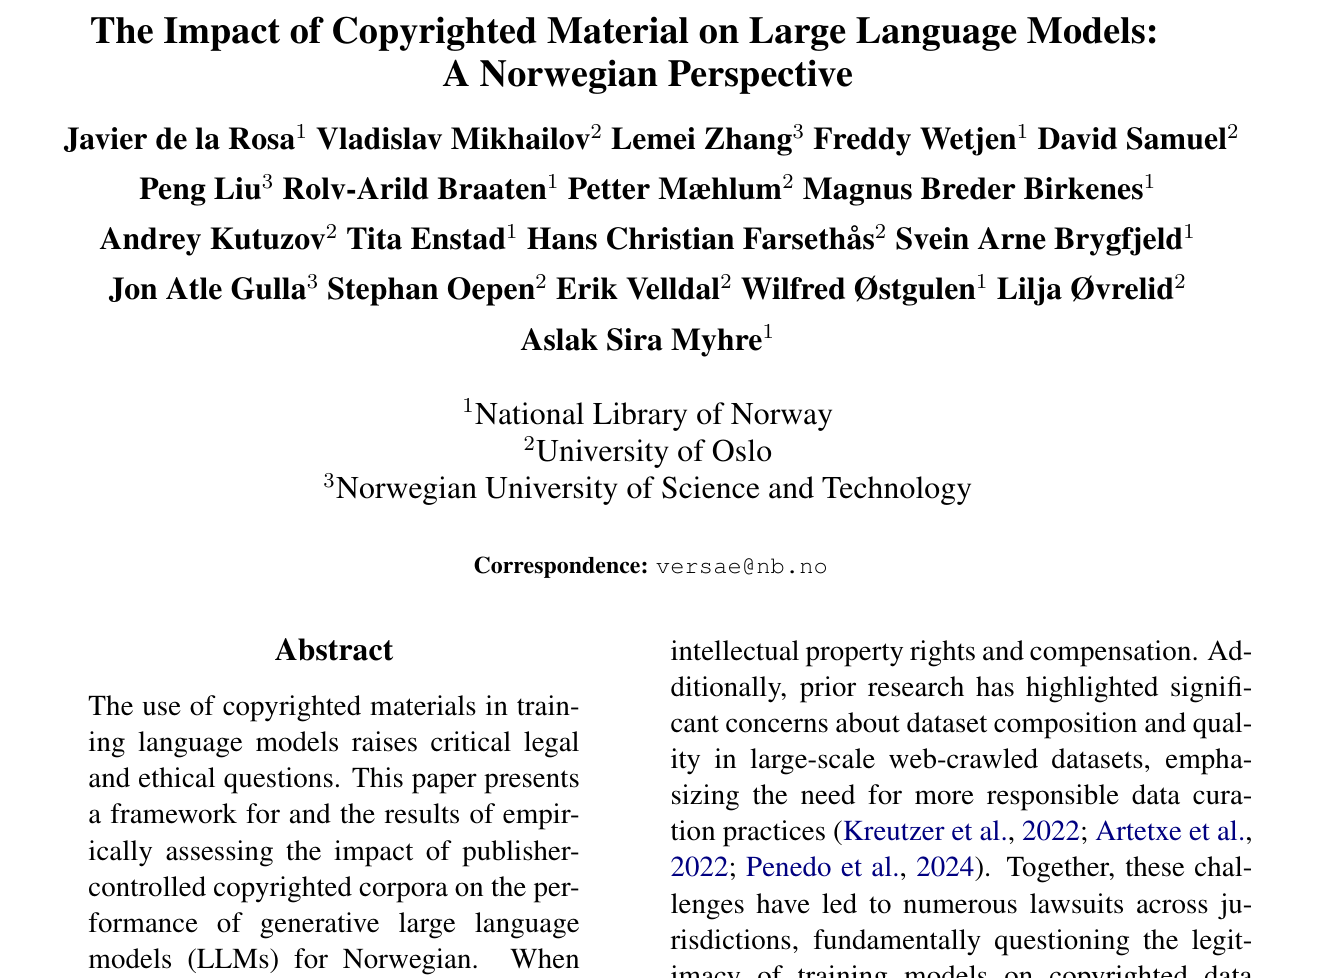
\includegraphics[width=.645\textwidth]{graphics/mimir}}\\[-.5ex]
    \color{DarkGreen}{\smaller\url{https://aclanthology.org/2025.nodalida-1.59/}}
  \end{center}
\end{frame}
\fi

\begin{frame}[fragile]\includelogo
  \frametitle{Det norske LLM-økosystemet i dag (som vi forstår det)}
  \pause
  \vskip 0ex
  \begin{block}{NTNU \& UiO (\& Nasjonalbiblioteket) -- Grunnleggende og anvendt forskning}
    \begin{center}
      \scshape\color{red}
      noe aktivitet i nasjonale og europeiske enkeltprosjekter;\\[.2ex]
      sterk fragmentering; ingen ki-senter har språkmodeller i fokus.
%      utfordrende for isolerte fagmiljøer å henge med internasjonalt.
    \end{center}
  \end{block}
  \pause
  \begin{block}{Nasjonalbiblioteket -- «Språkmodellfabrikken»}
    \begin{center}
      \scshape\color{DarkBlue}
      utvikling av «produksjons»-modeller for norsk og samiske språk;\\[.2ex]
      statsbudsjett {\smaller 2025 \& 2026}:\ grunnbevilgning, dog ikke forskning.
    \end{center}
  \end{block}
  \pause
  %
  % https://www.forskningsradet.no/nyheter/2025/investere-milliarder-infrastruktur-tungregning/
  %
  \begin{block}{Sigma2 -- Styrket GPU-kapasitet og tungregningskompetanse}
    \begin{center}
      \scshape\color{DarkBlue}
      storskala forskningsinfrastruktur avgjørende llm-drivkraft;
      sammenlignet med finland eller sveits ligger norge langt bak.
    \end{center}
  \end{block}
  \pause
  \begin{block}{KI Norge \& \textit{New Nordics AI} -- KI-basert innovasjon, tilsyn, regulering}
    \begin{center}
      \scshape\color{DarkBlue}
%      ansvarlig ki-utvikling og -bruk i offentlig og privat sektor;\\[.2ex]
      bred tolkning av ki; ikke fokus på forskning eller språkmodeller.
    \end{center}
  \end{block}
\end{frame}

\begin{frame}[fragile]\includelogo
  \frametitle{8.\ juni:\ Nasjonal statusmelding og «Klyngas anbefalinger»}
  \vskip -1ex
  \begin{columns}
    \begin{column}{.6\textwidth}
      \begin{center}
        \fbox{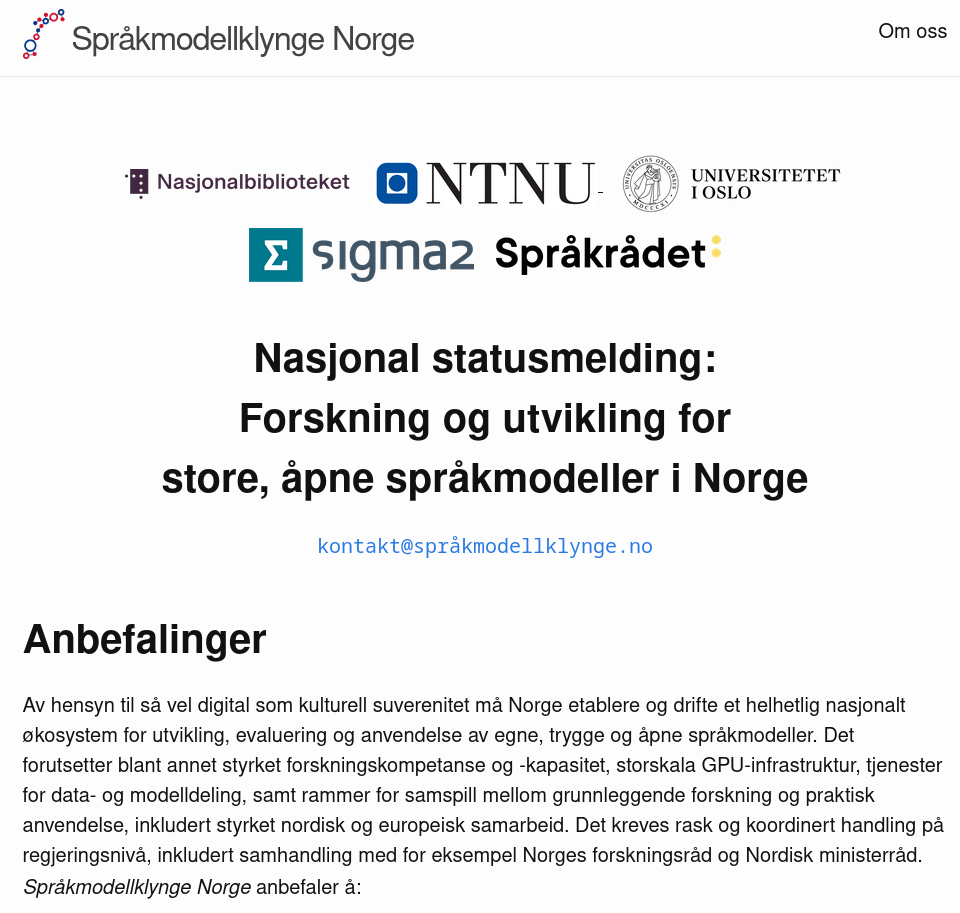
\includegraphics[width=.86\textwidth]{graphics/anbefalinger}}\\[1.5ex]
      \end{center}
    \end{column}
    \begin{column}{.4\textwidth}
      \begin{center}
        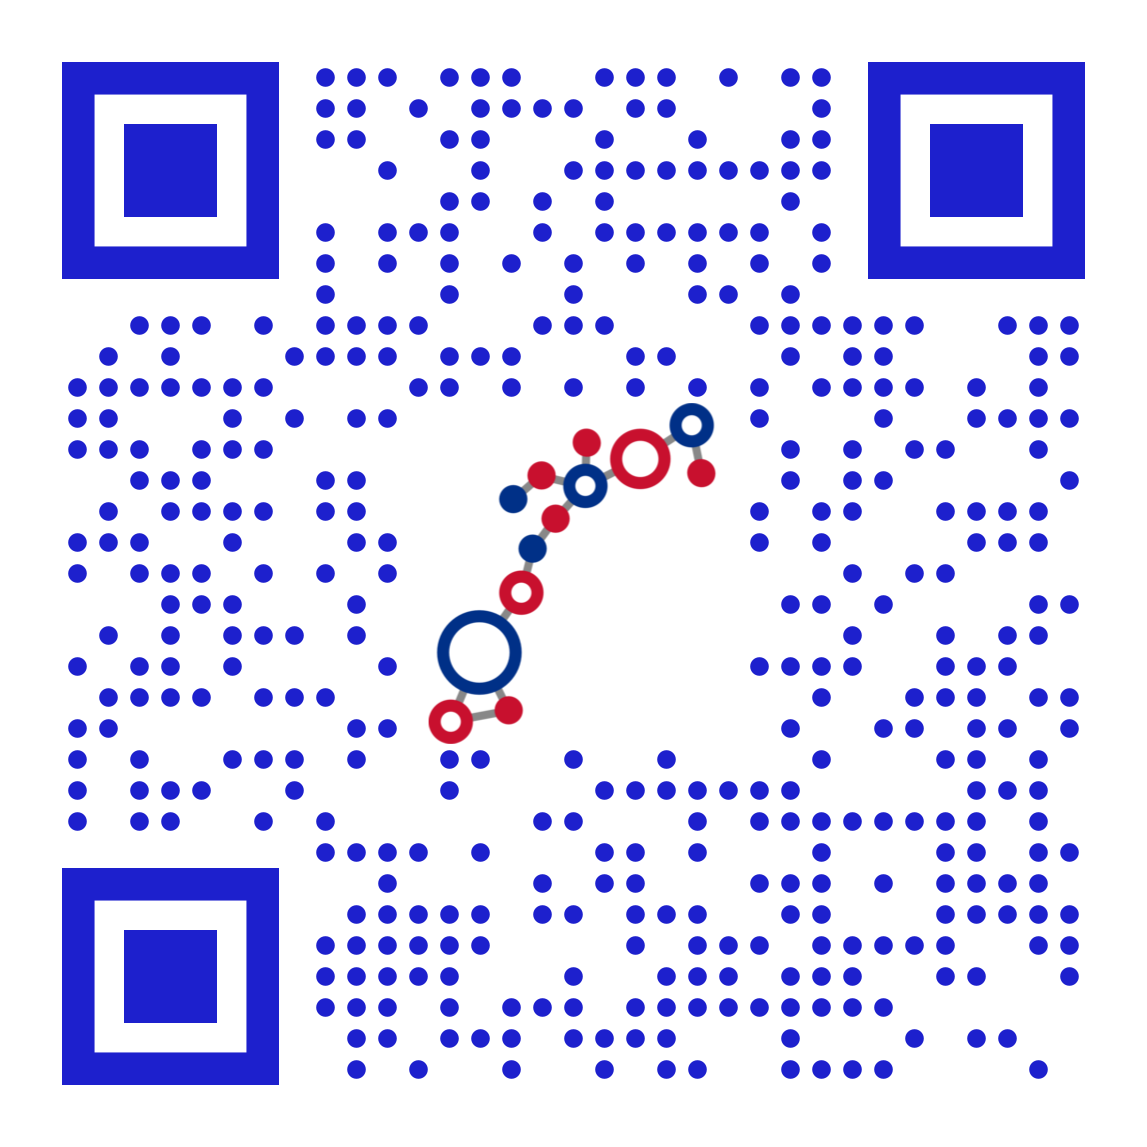
\includegraphics[width=\textwidth]{graphics/qr}\\[.5ex]
        \color{DarkGreen}{\smaller[3]\url{https://spr\aa kmodellklynge.no/}}\\
      \end{center}
    \end{column}
  \end{columns}
\end{frame}

\begin{frame}[fragile]\includelogo
  \frametitle{Klyngas anbefalinger (1 av 2)}
  \pause
  \vskip 1ex
  \begin{block}{}
    \color{DarkBlue}
    \raisebox{-1ex}{\Huge 1.}\hskip 1em
    \parbox{0.9\textwidth}{%
      Igangsette en \alert{hurtigarbeidende prosess mot en helhetlig nasjonal LLM-strategi},
      med reell involvering av de sentrale norske forskningsmiljøene sammen med øvrige nasjonale aktører.}
  \end{block}
  \pause\vskip 1ex
  \begin{block}{}
    \color{DarkBlue}
    \raisebox{-1ex}{\Huge 2.}\hskip 1em
    \parbox{0.9\textwidth}{%
      Etablere et \alert{nasjonalt KI-forskningsenter for åpne språkmodeller}
      som samler aktørene i et faglig fellesskap, med en tilhørende \alert{forskerskole}.
      I et femårsperspektiv bør det utdannes \alert{15–20 doktorgrader}.}
  \end{block}
  \pause\vskip 1ex
  \begin{block}{}
    \color{DarkBlue}
    \raisebox{-1ex}{\Huge 3.}\hskip 1em
    \parbox{0.9\textwidth}{%
      \alert{Videreutvikle Sigma2} som nasjonal leverandør av regnekraft,
      LLM-tjenester og tungregningskompetanse, herunder
      \alert{utvidet norsk engasjement i europeiske tungregningsinfrastrukturer} som LUMI-AIF og EuroHPC.}
  \end{block}
\end{frame}

\begin{frame}[fragile]\includelogo
  \frametitle{Klyngas anbefalinger (2 av 2)}
  \vskip 1ex
  \begin{block}{}
    \color{DarkBlue}
    \raisebox{-1ex}{\Huge 4.}\hskip 1em
    \parbox{0.9\textwidth}{%
      Stimulere til \alert{nordisk forsknings- og utviklingssamarbeid} gjennom blant annet
      data- og modelldeling, forskermobilitet, koordinert forskerutdanning,
      en \alert{årlig nordisk møteplass for forskere og utviklere} av åpne språkmodeller.}
  \end{block}
  \pause\vskip 1ex
  \begin{block}{}
    \color{DarkBlue}
    \raisebox{-1ex}{\Huge 5.}\hskip 1em
    \parbox{0.9\textwidth}{%
      Utvikle \alert{rettslige og praktiske rammer} for datadeling,
      som balanserer opphavsrett og personvern med behovene for \alert{trening
      på storskala data} og for \alert{inspeksjon og validering} av modeller.}
  \end{block}
  \pause\vskip 1ex
  \begin{block}{}
    \color{DarkBlue}
    \raisebox{-1ex}{\Huge 6.}\hskip 1em
    \parbox{0.9\textwidth}{%
      Etablere norsk medlemskap i det \alert{europeiske \textit{Alliance for Language Technologies}}
      (ALT-EDIC) og økonomiske rammer for deltakelse fra universitetsmiljøer i
      \alert{\textit{Digital Europe}--programmet}.}
  \end{block}
\end{frame}

\begin{frame}[fragile]\includelogo
  \frametitle{Veien videre:\ Klyngas aktiviteter i 2026}
  \pause
  \vskip .5ex
  \begin{block}{Flere FoU-medlemmer og observatører}
    \begin{center}
      \scshape\color{DarkBlue}
      samiske fagmiljøer ved sámi allaskuvla og uit;\\
      uib, uis, nr, simula, \ldots; ki norge.\\[.5ex]
    \end{center}
  \end{block}
  \pause
  \vskip .5ex
  \begin{block}{Felles forskningsinfrastruktur:\ data, evaluering, programvare}
    \begin{center}
      \scshape\color{DarkBlue}
      enhetlig oppsett på olivia og lumi; standardisert evaluering;\\[.5ex]
      samarbeid med alt-edic:\ norsk instans av compar:ia-arena.\\[.5ex]
    \end{center}
  \end{block}
  \pause
  \begin{block}{30.\ november \& 1.\ desember:\ \textit{Nordic LLM Summit}}
    \begin{center}
      \scshape\color{DarkBlue}
      30--40 forskere fra danmark, island, finland, sverige:\ «hands-on»;\\
      koordinering, mulig samarbeid, f.eks.\ datadeling, evaluering.\\[.5ex]
    \end{center}
  \end{block}
  \vskip 1ex
  \centerline{\raisebox{1ex}{\color{DarkBlue}\bf\ldots}}
\end{frame}

\begin{frame}[fragile,plain]
  \begin{columns}
    \begin{column}{0.4\textwidth}
      \vspace*{-8ex}
      \begin{center}
        \fontsize{7cm}{7cm}\selectfont\bfseries 2
      \end{center}      
    \end{column}
    \begin{column}{0.65\textwidth}
      \begin{center}\renewcommand{\baselinestretch}{1.5}
        \fontsize{1.1cm}{1.1cm}\selectfont\bfseries
        Over There\\ in Europe
      \end{center}
    \end{column}
  \end{columns}
\end{frame}

\begin{frame}[fragile]\includeopeneurollm
  \frametitle{For eksempel:\ Europas største FoU-initiativ på området}
  \vskip 1ex
  \begin{center}
    
\includegraphics[width=.7\textwidth]{graphics/openeurollm}\\[0.5ex]
  \end{center}
\end{frame}

\begin{frame}[fragile]\includeopeneurollm % oe
  \frametitle{The Consortium:\ 21 Partners, 9 European Countries}
  \begin{center}
    \vspace*{-2.5ex}
    \fboxsep 0pt
    \fbox{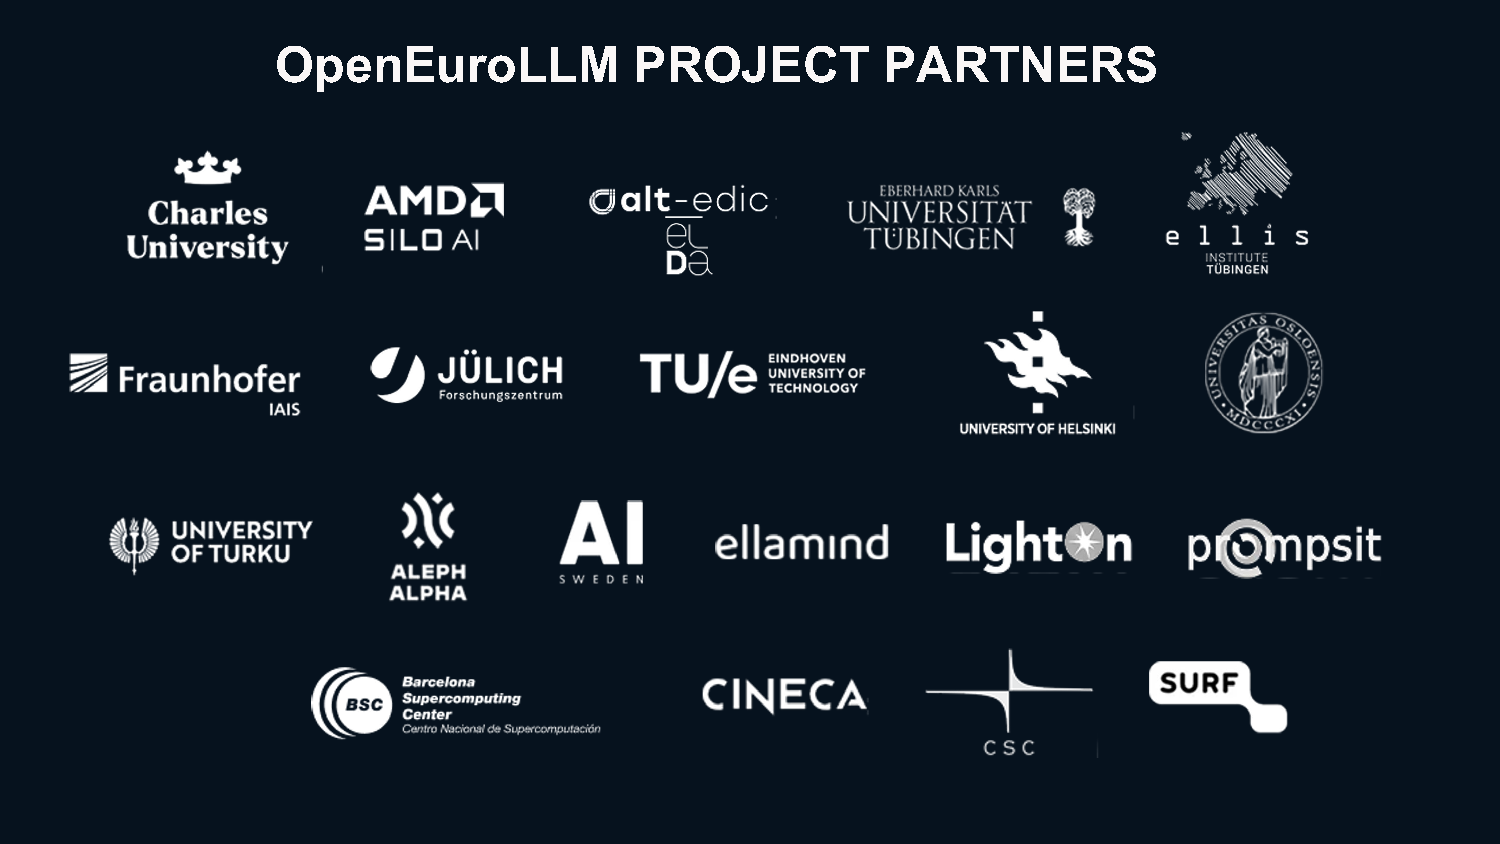
\includegraphics[width=\textwidth, page=1, trim={0.6cm 1cm 1.5cm 2cm}, clip]{consortium}}\\[1ex]
  \end{center}
\end{frame}

\begin{frame}[fragile]\includeopeneurollm % oe
  \frametitle{The Consortium:\ 21 Partners, 9 European Countries}
  \begin{center}
    \vspace*{-2.5ex}
    \fboxsep 0pt
    \fbox{\includegraphics[width=\textwidth, page=2, trim={0.6cm 1cm 1.5cm 2cm}, clip]{consortium}}\\[1ex]
  \end{center}
\end{frame}

\begin{frame}[fragile]\includeopeneurollm % oe
  \frametitle{The Consortium:\ 21 Partners, 9 European Countries}
  \begin{center}
    \vspace*{-2.5ex}
    \fboxsep 0pt
    \fbox{\includegraphics[width=\textwidth, page=3, trim={0.6cm 1cm 1.5cm 2cm}, clip]{consortium}}\\[1ex]
  \end{center}
\end{frame}

\begin{frame}[fragile]\includeopeneurollm % oe
  \frametitle{The Consortium:\ 21 Partners, 9 European Countries}
  \begin{center}
    \vspace*{-2.5ex}
    \fboxsep 0pt
    \fbox{\includegraphics[width=\textwidth, page=4, trim={0.6cm 1cm 1.5cm 2cm}, clip]{consortium}}\\[1ex]
  \end{center}
\end{frame}

\begin{frame}[fragile]\includeopeneurollm % oe
  \frametitle{The Mission: Digital Sovereignity -- Transparent AI}
  \pause
  \begin{block}{Linguistic Equity}
    \begin{center}\color{DarkGreen}
      \alert{36$^+$ languages}:\ member states, candidate members, close associates;\\[0.5ex]
      emphasize \alert{multilingual evaluation}:\ new datasets and benchmarks.
    \end{center}
  \end{block}
  \pause
  \begin{block}{Open Models \& Data}
    \begin{center}\color{DarkBlue}
      Share models under \alert{permissive open-source licenses} (e.g.\ Apache 2.0);\\[0.5ex]
      make \alert{complete and exact training data} generally available for verification.
    \end{center}
  \end{block}
  \pause
  \begin{block}{Verifiable Openness}
    \begin{center}\color{DarkGreen}
      Open-source \& document \alert{full pipeline}:\ code, recipes, results.
    \end{center}
  \end{block}
  \pause
  \begin{block}{Reusable Infrastructure}
    \begin{center}\color{DarkBlue}
      Uniform data management, tools, workflows across EuroHPC ecosystem.
    \end{center}
  \end{block}
\end{frame}

\begin{frame}[fragile]\includeopeneurollm % oe
  \frametitle{Project Lifecycle:\ Preparation -- Production -- Flagship}
  \begin{center}
    \vspace*{1ex}
    \fboxsep 0pt
    \fbox{\includegraphics[width=.97\textwidth, page=2, trim={0.5cm 1.5cm 0.5cm 2.5cm}, clip]{gema}}\\[2.5ex]
    \scshape
    \textcolor{DarkBlue}{collaboration} --
    \textcolor{DarkGreen}{data mixtures} --
    \textcolor{DarkBlue}{infrastructure} --
    \textcolor{DarkGreen}{evaluation}
  \end{center}
\end{frame}

\begin{frame}[fragile]\includeopeneurollm % oe
  \frametitle{The Quest for Compute}
  \begin{center}
    \vspace*{-.5ex}
    \fboxsep 0pt
    \fbox{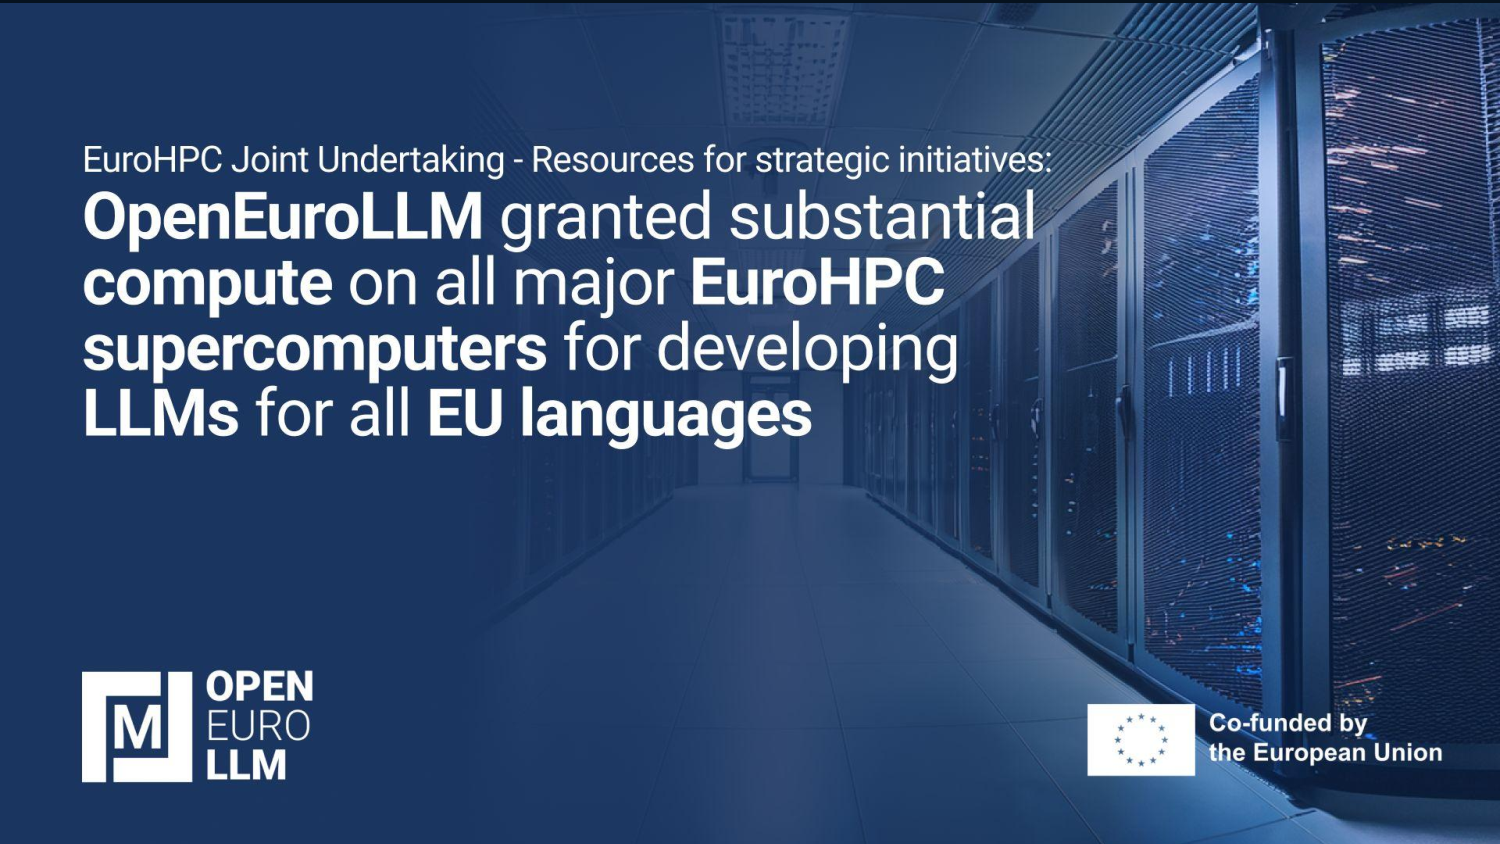
\includegraphics[width=.99\textwidth, page=1, trim={0cm 0cm 0cm 1.3cm}, clip]{gema}}\\[1ex]
  \end{center}
\end{frame}

\begin{frame}[fragile]\includelogo
  \frametitle{Regnekraft, nok en gang:\ OpenEuroLLMs GPU-kalkulator}
  \vskip -1ex
  \begin{center}
    \fbox{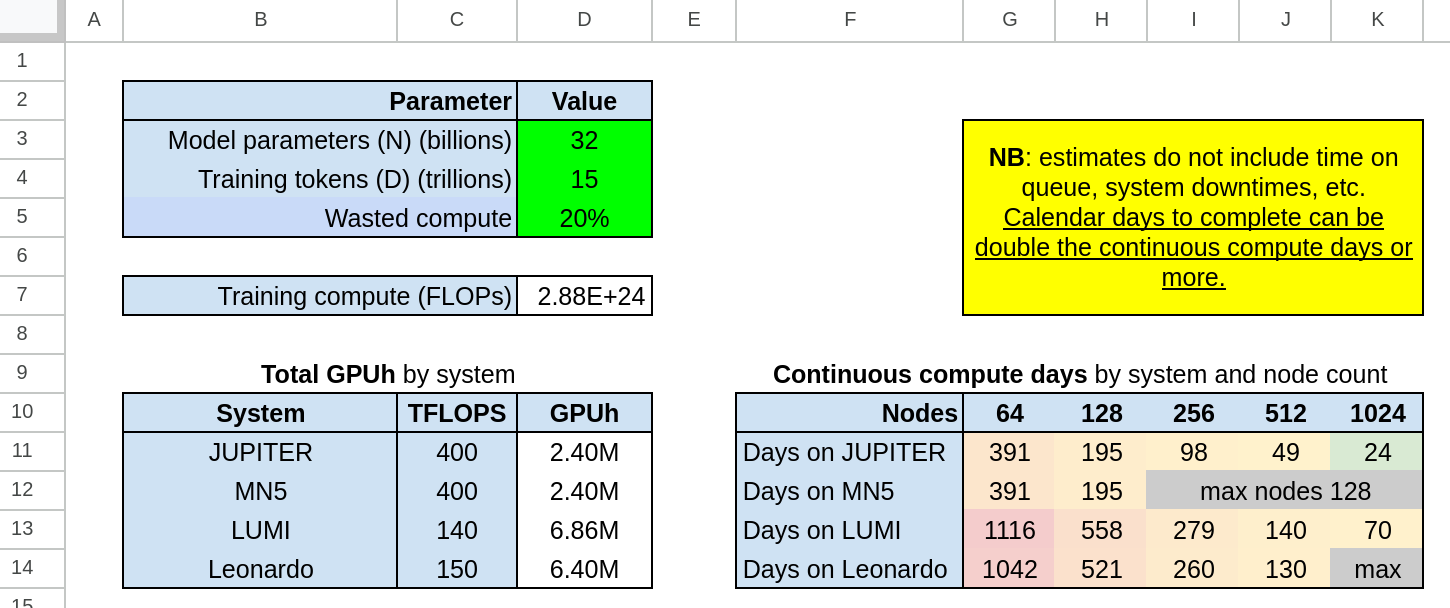
\includegraphics[width=.9\textwidth]{graphics/kalkulator}}
  \end{center}
  \vskip -.5ex
  \begin{block}{}
    \begin{center}
      \scshape\color{red}
      grunntrening av mellomstor modell krever europeisk samarbeid;\\[.2ex]
      (eller en satsing à la sveits; olivia er om lag {\smaller 1/24}-del av alps).
    \end{center}
  \end{block}
\end{frame}

\begin{frame}[fragile,plain]
  \begin{columns}
    \begin{column}{0.4\textwidth}
      \vspace*{-8ex}
      \begin{center}
        \fontsize{7cm}{7cm}\selectfont\bfseries 3
      \end{center}      
    \end{column}
    \begin{column}{0.65\textwidth}
      \begin{center}\renewcommand{\baselinestretch}{1.5}
        \fontsize{1.1cm}{1.1cm}\selectfont\bfseries
        Norwegian in\\ OpenEuroLLM
      \end{center}
    \end{column}
  \end{columns}
\end{frame}

%
% a little less than 50b tokens for both languages;
% nynorsk heavily upsampled (up to factor of ten);
% nynorsk about 40% of total
%
\begin{frame}[fragile]\includeopeneurollm % oe
  \frametitle{2025 Pretraining Data Mix:\ 10 Trillion Tokens}
  \vskip -1ex
  \begin{center}
    \fbox{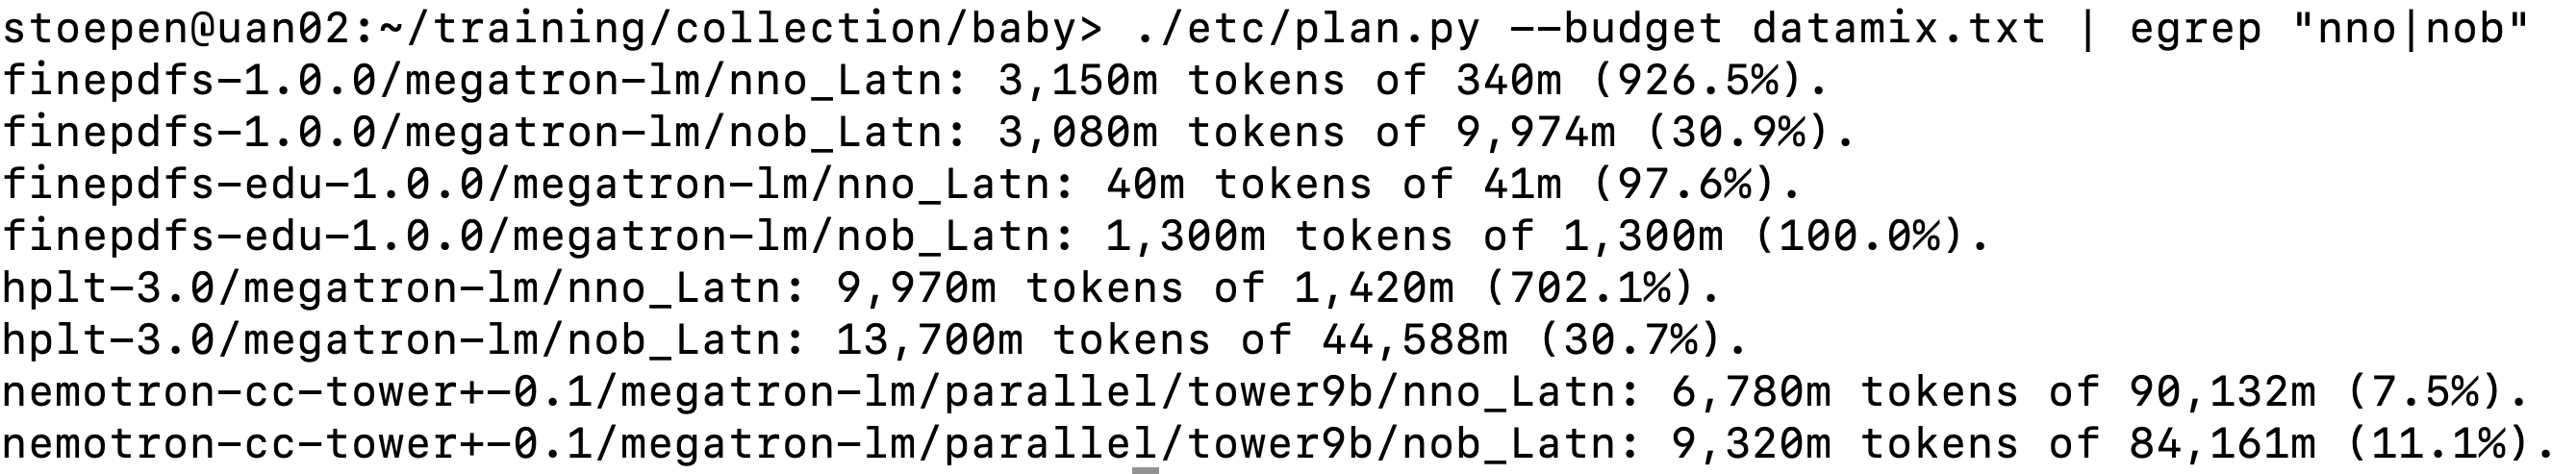
\includegraphics[width=.98\textwidth]{graphics/baby}}
  \end{center}
  \vskip -1ex
  \begin{block}{Norwegian:\ \textit{Bokmål} and \textit{Nynorsk}}
    \begin{center}
      \vskip .5ex
      \scshape\color{DarkBlue}
      close to {\smaller 50}b tokens for both languages:\ about {\smaller 0.5} percent;\\[0.3ex]
      about {\smaller 40} percent nynorsk; heavily upsampled (up to ten times);\\[0.3ex]
      using all available nynorsk, but only about {\smaller 1/3} of all bokmål;\\[0.3ex]
      one third of data ({\smaller 17}b tokens) machine translated from english.
    \end{center}
  \end{block}
  \pause
  \vskip .5ex
  \centerline{\scshape\color{red} english-first pretraining as best practice -- ``general capabilities''}
\end{frame}

\begin{frame}[fragile,c]
  \frametitle{For Example, Translating from ``High-Quality'' English}
  \vskip -1ex
  \begin{columns}
    \begin{column}{.28\textwidth}
      \begin{center}
        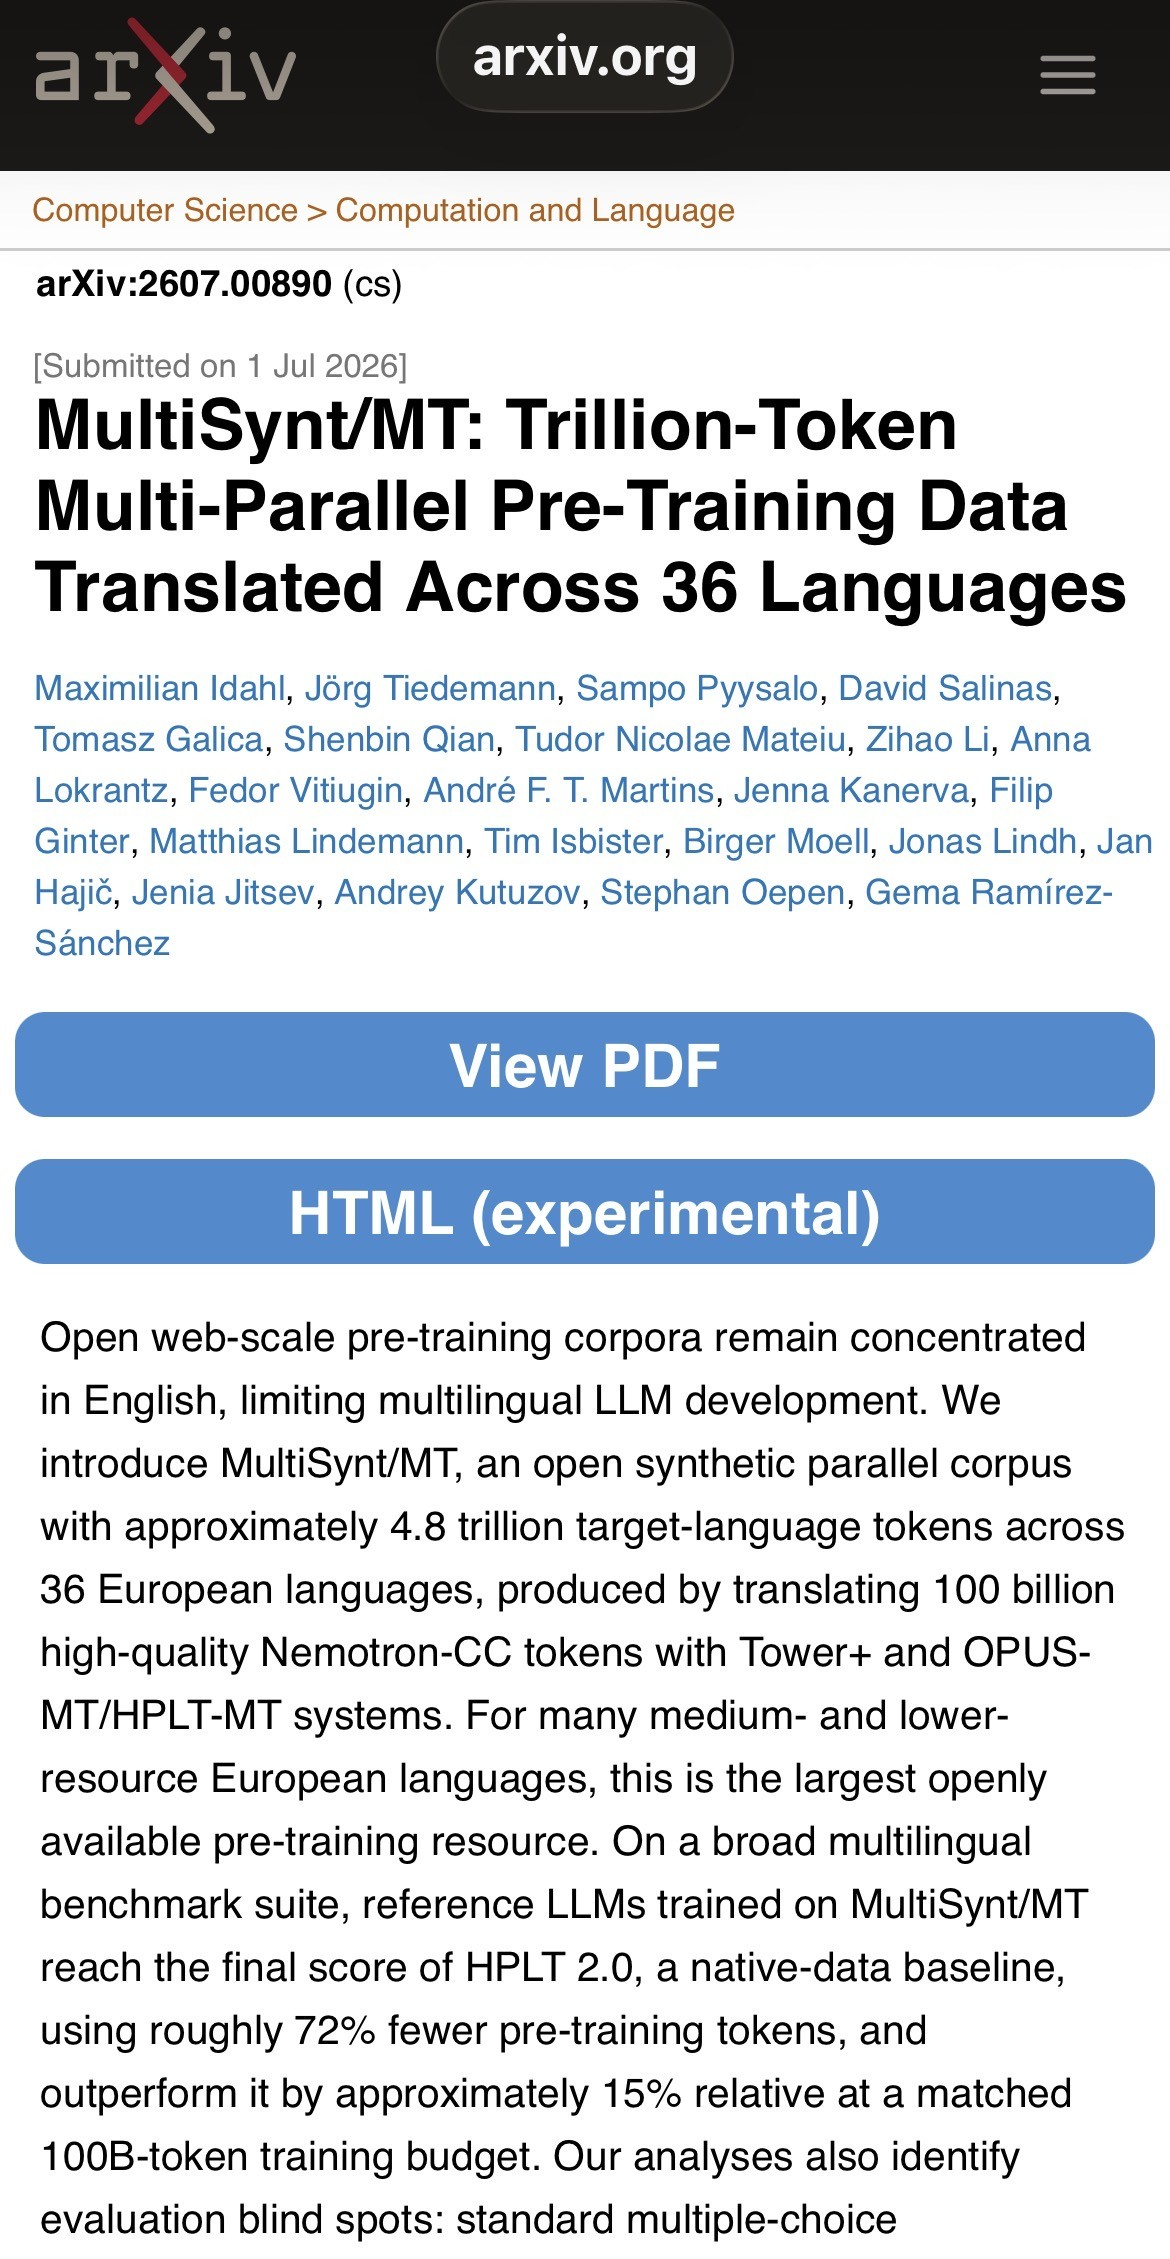
\includegraphics[width=.92\textwidth]{graphics/multisynt-mt}
      \end{center}      
    \end{column}
    \begin{column}{.72\textwidth}
      \begin{center}
        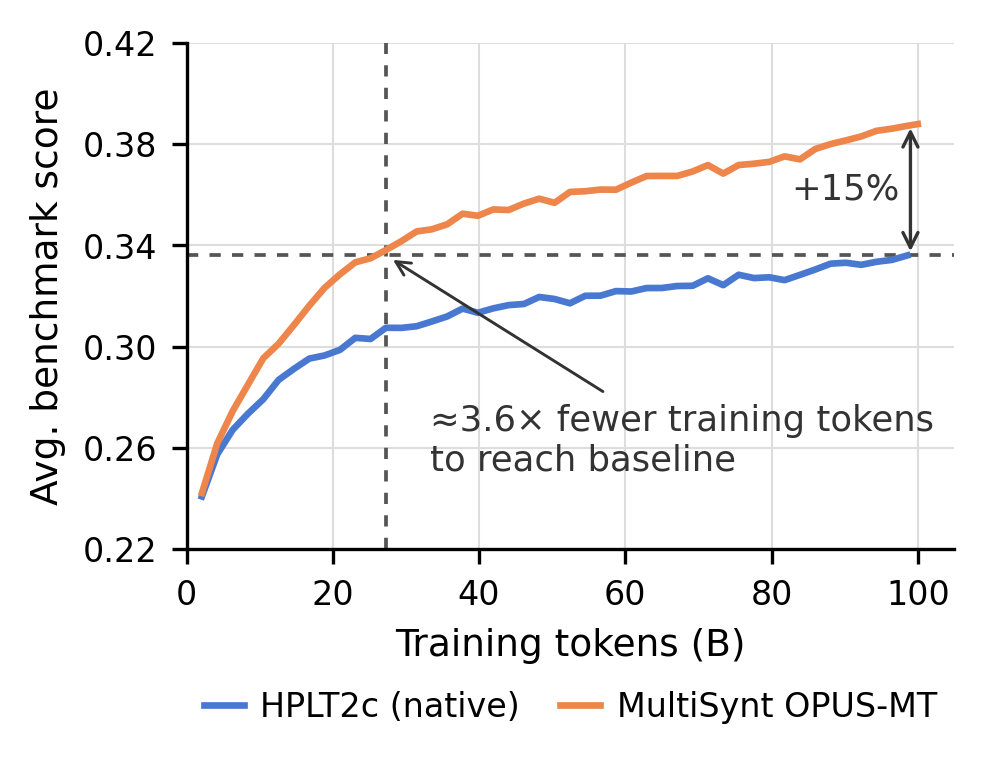
\includegraphics[width=.8\textwidth]{graphics/gains-compute}\\[1ex]
        \textcolor{DarkGreen}{\url{https://arxiv.org/abs/2607.00890}}
      \end{center}
    \end{column}
  \end{columns}
\end{frame}

\begin{frame}[fragile]\includelogo
  \frametitle{Your Mileage May Vary}
  \vskip 10ex
  \begin{center}
    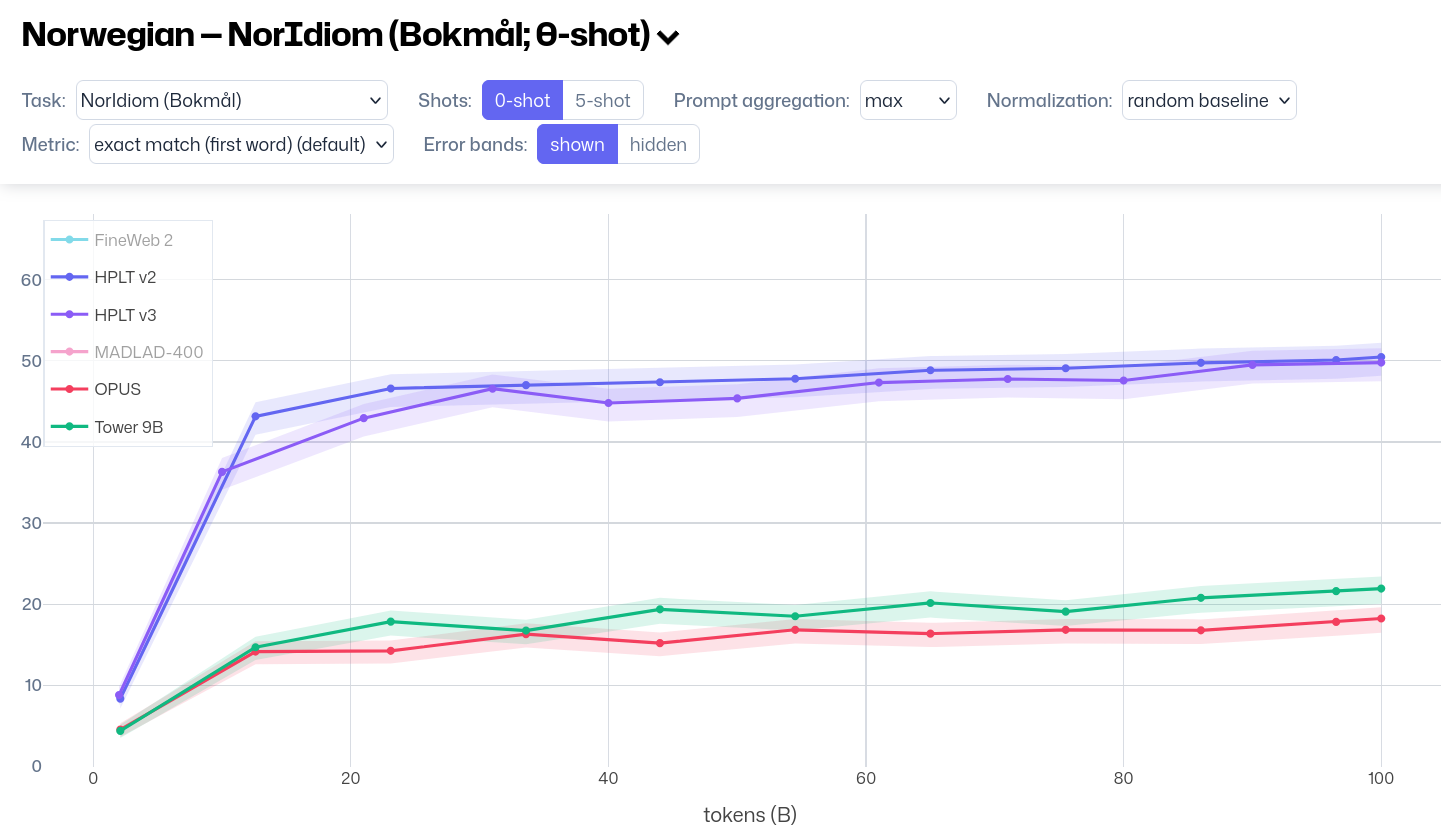
\includegraphics[width=.48\textwidth]{graphics/noridiom_nob}\hfill
    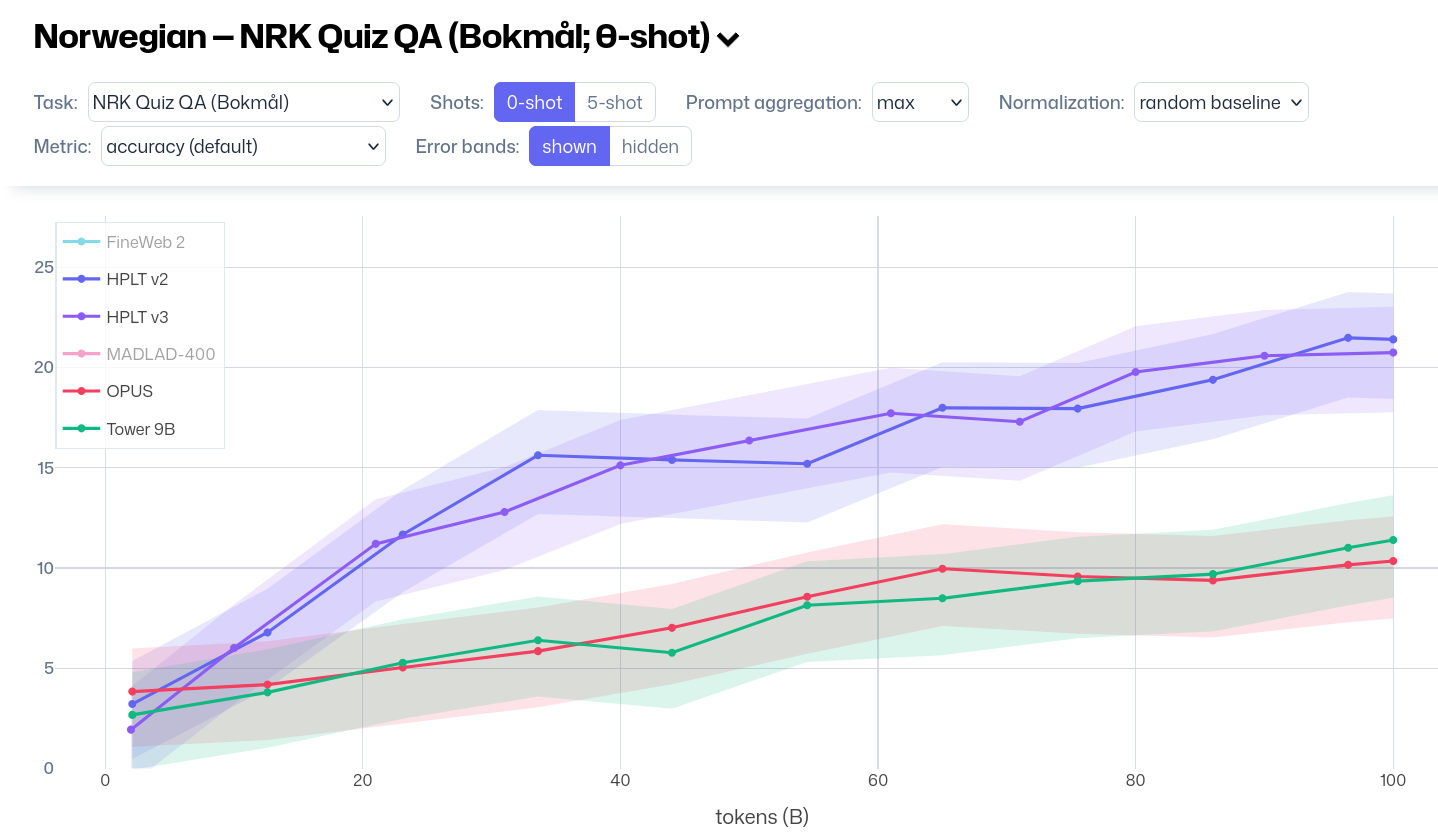
\includegraphics[width=.48\textwidth]{graphics/nrkqa_nob}\\[5ex]
    {\color{DarkGreen}\url{https://ltgoslo.github.io/llm-dashboard/multisynt/?lang=Norwegian}}
  \end{center}
\end{frame}

\begin{frame}[fragile,plain]
  \begin{columns}
    \begin{column}{0.4\textwidth}
      \vspace*{-8ex}
      \begin{center}
        \fontsize{7cm}{7cm}\selectfont\bfseries 4
      \end{center}      
    \end{column}
    \begin{column}{0.65\textwidth}
      \begin{center}\renewcommand{\baselinestretch}{1.5}
        \fontsize{1.1cm}{1.1cm}\selectfont\bfseries
        Wrap-Up\\ Outlook
      \end{center}
    \end{column}
  \end{columns}
\end{frame}

\begin{frame}[fragile]\includelogo
  \frametitle{A Handful of Overarching Reflections}
\end{frame}

\begin{frame}[fragile]\includelogo
  \frametitle{Sveits, for eksempel:\ Alps \& Apertus}
  \vskip 2ex
  \begin{columns}
    \begin{column}{.5\textwidth}
      \begin{center}
        \fbox{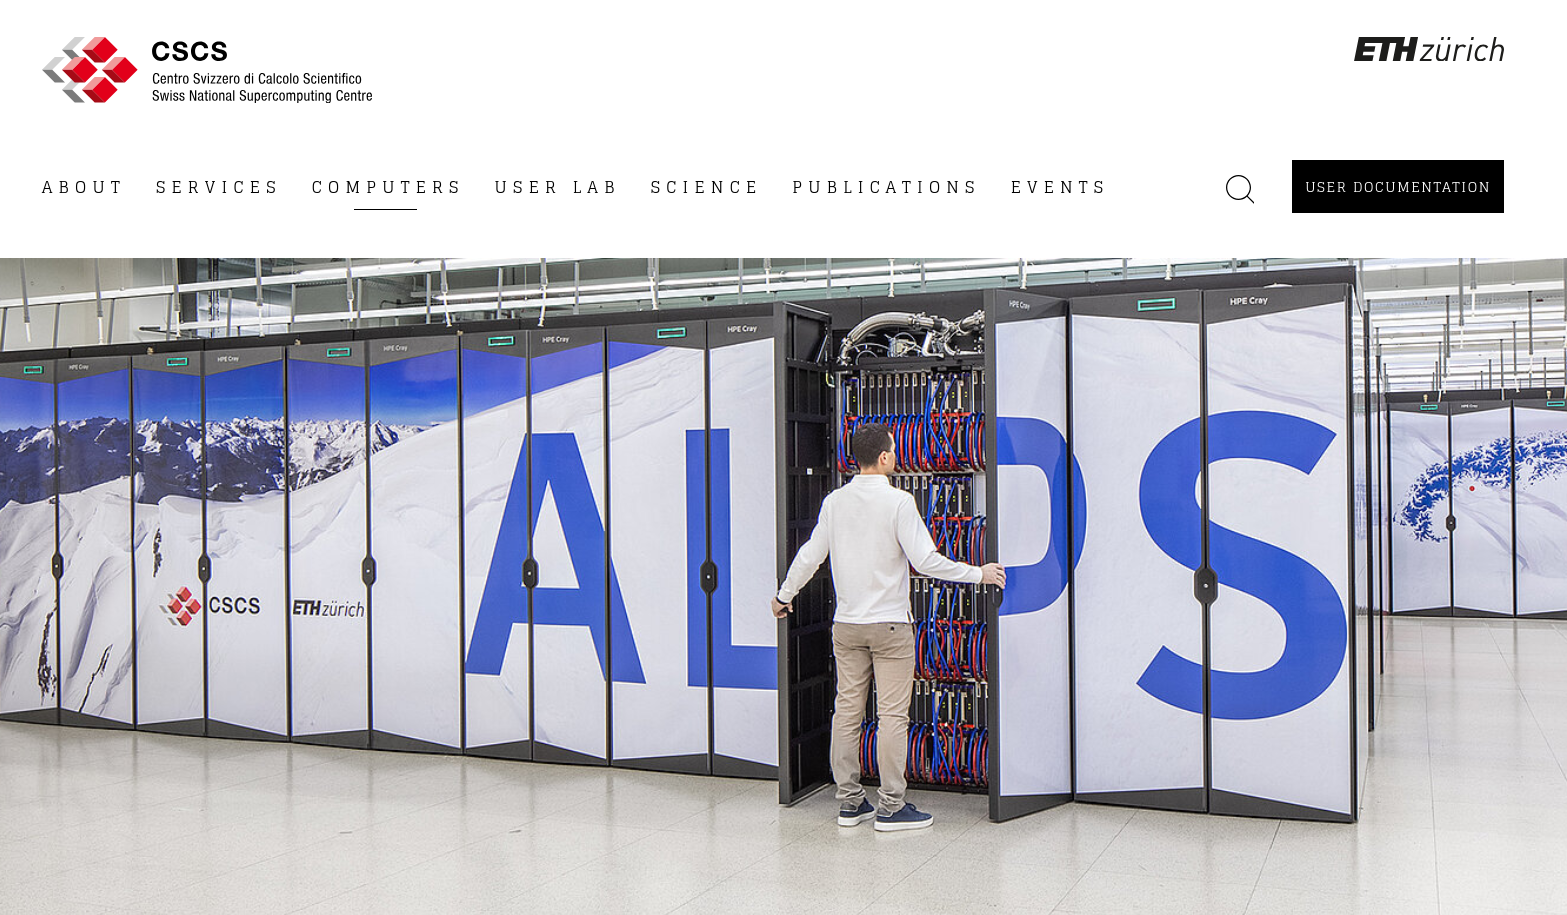
\includegraphics[width=.95\textwidth]{graphics/alps}}\\[1.5ex]
      \end{center}
    \end{column}
    \begin{column}{.5\textwidth}
      \begin{center}
        \fbox{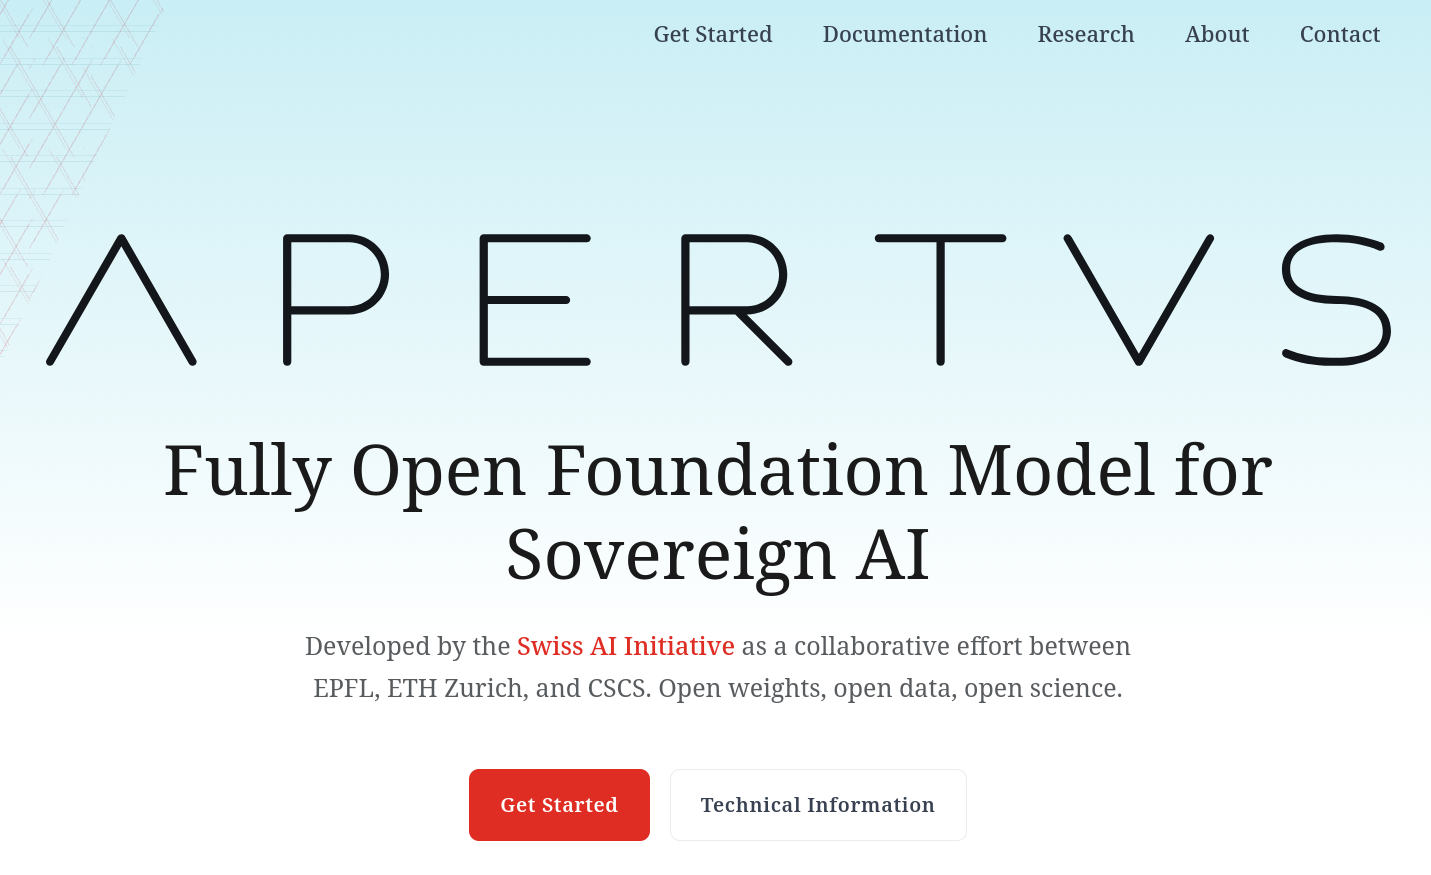
\includegraphics[width=.95\textwidth]{graphics/apertus}}\\[1.5ex]
      \end{center}
    \end{column}
  \end{columns}
  \pause
  \vskip 5ex
  \begin{center}
    \begin{center}
      \scshape\color{DarkBlue}
      three sites (eth, epfl, cscs):\ cohesive team; \alert{prioritized gpu access};\\[.8ex]
      currently strongest \alert{fully open}, \alert{multilingual} models ({\smaller 9}b \& {\smaller 70}b).
    \end{center}    
  \end{center}
\end{frame}

\begin{frame}[fragile]\includelogo
  \frametitle{Kontakt}
  \vskip 1ex
  \begin{center}
    \color{DarkGreen}
    \textbf{Stephan Oepen}\\[1ex]
    Language Technology Group\\
    University of Oslo\\[0.5ex]
    \texttt{oe@ifi.uio.no}\\[3ex]
    \fbox{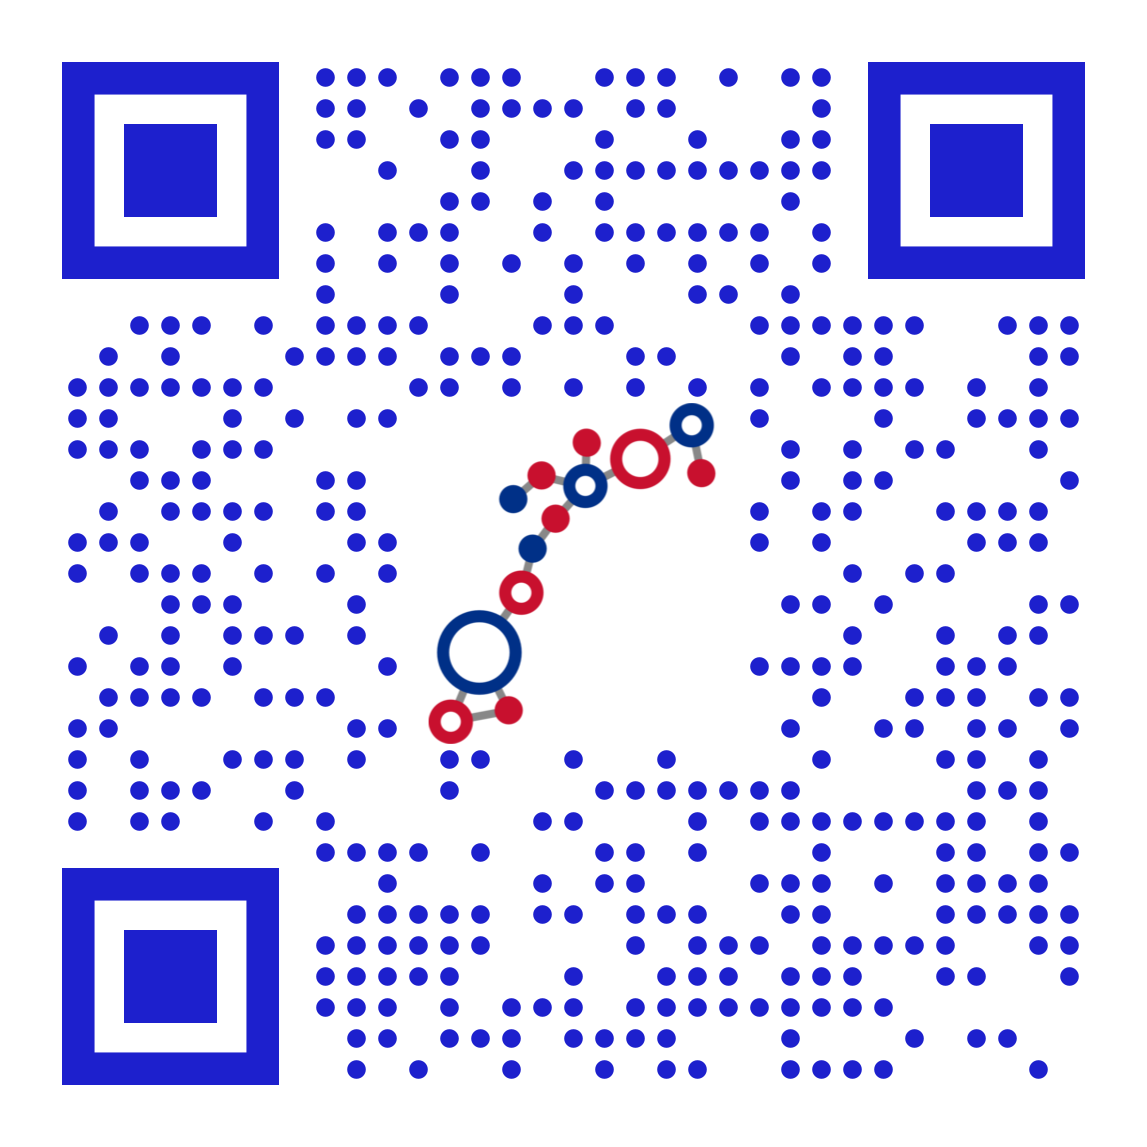
\includegraphics[height=20ex]{graphics/qr}}\\
    \textcolor{DarkGreen}{\url{https://spr\aa kmodellklynge.no/}}\\
    \textcolor{DarkGreen}{\url{https://www.openeurollm.eu//}}
  \end{center}
\end{frame}


\end{document}
